\subsection{モデルの説明}
このモデルでは,3.2で考えたモデルと同様に,点$x$をそれまでに選択された点からの近さで選んでゆくようなモデルを考えることにする。

これまで考えてきたモデルとの大きな相違は,点を選択していく過程をは始める前に,すべての$x$について,自分から近い位置にある点同士をエッジで結んでいき,クラスターを形成することである。こうして得られたクラスター$y$について,その一つ前に選ばれた点$x$から最も近い点を含む$y$から,次の時刻の点が選ばれるとする。このとき$y$の中から点を選ぶ方法は,そのクラスター内に含まれる点の属するそれぞれの$X$に割り当てられた重みによって決定されるとする。

このモデルの着想を得るにあたって,実際の話し合いの際に,人が多くなることによって人がどのように考えるか,ということに影響を受けている。すなわち,話し合いに参加する人が多いほど,自分の意見と同じ様な意見をもつ人がいるだろう,と思う効果であり,$X_{i}$に割り当てられた重みは,個人の発言力をあらわしていると考えることができる。

シミュレーションにおいてクラスター化を行う際には,自分と他の点との間の距離を測り,これが$r$より小さいものの間にエッジを張ることにする。このとき,(特に$r$が小さいときに)効率よく近傍点を探すことができるよう,はじめに全体を長さ$l(>r)$の正方形の領域(セル)に分割し,それぞれの点がどのセルに属しているかを記録しておく。このようにすると,近傍点を探す際には,自分の属するセルとその周囲8マスを含めた9つのセルの中にある点のみについて調べればよい。このようにしてすべての点について順番に閾値$r$の内部にある点を選択していく。このとき領域内に入ったすべての点にクラスター番号が与えられていない時には,通し番号でクラスター番号を割り当てる。閾値$r$で定められる領域内に,より小さいクラスター番号をもつ点が存在する時には,その中で一番小さいクラスター番号を,接続しているすべての点に同じクラスター番号を付与する。このようにすれば,既に存在するクラスターとの間の融合などを考慮に入れたクラスター化が行える。また,今回のシミュレーションでは,$X_{i}$の違いによる選択確率の違いはないものとした。

\subsection{シミュレーション結果}
図\ref{fig:f15}に,$r=0.07, K=20, N=4, S=20$としたときに実際にどのようにクラスターが形成され,点が選択されていくかの様子を示した図を載せる。グラフで薄いグレーで描かれた線はノード間の距離が$r$より小さいために張られたエッジであり,これが連結しているひとまとまりがクラスターである。青色の線は,選ばれた点同士をつなぐ(有向)エッジであり,振られている番号は時刻$k$に張られたエッジであることを表す。
\begin{figure}[H]
    \begin{center}
        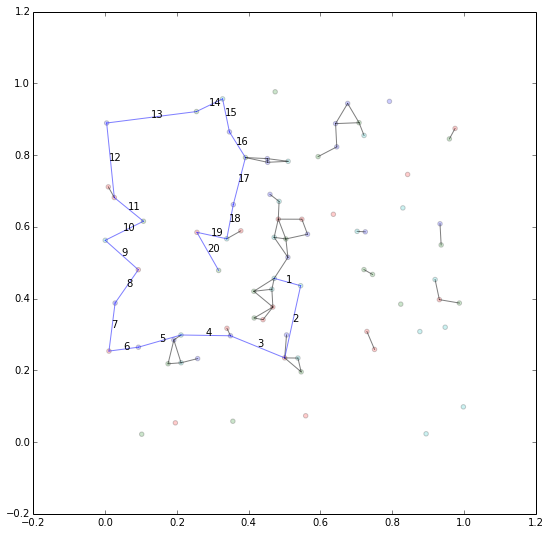
\includegraphics[width=10cm]{../img/cluster.png}
        \caption{近傍点をクラスター化するモデルのシミュレーション結果の例}
        \label{fig:f15}
    \end{center}
\end{figure}

このシミュレーションでは,考えるべき問題が二つある。一つは$r$によって作られるクラスターに関する性質である。もうひとつは,選ばれた点によって作られた軌跡に関するものだである。ただし,それぞれが独立でないために,完全に分けて考えることはできない。

まずは,閾値$r$と,点の密度に関係してクラスターがどのように形成されるかについての議論をしていくことにする。図\ref{fig:f16}は閾値$r$を変えたときの,点の総数に対するクラスターの数の関係を示している。横軸$r$,縦軸$\phi = 1- (\text{クラスターの数})/(\text{点の総数})$として,通常の軸でのプロット(上段)と両対数プロット(下段)を取っており,縦軸の値は100回の試行の平均をとったものとなっている。
\begin{figure}[H]
    \begin{center}
        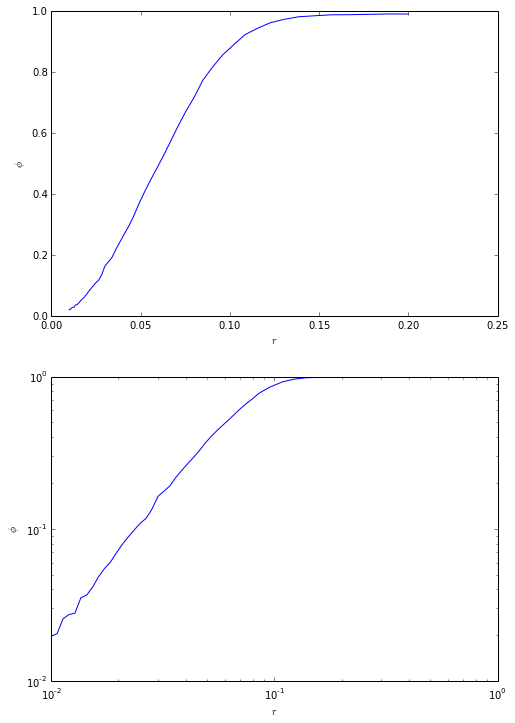
\includegraphics[width=10cm]{../img/r_phi_1.png}
        \caption{横軸$r$,縦軸$\phi = 1- (\text{クラスターの数})/(\text{点の総数})$としたグラフ}
        \label{fig:f16}
    \end{center}
\end{figure}
両対数プロットを見て分かるように,$r$の小さい領域では,ベキで近似することができそうであることが分かる。図\ref{fig:f17}には,この両対数グラフの$0<r<0.07$の範囲を直線でフィッティングしたものを示す。このときの傾きは,およそ1.86であった。
\begin{figure}[H]
    \begin{center}
        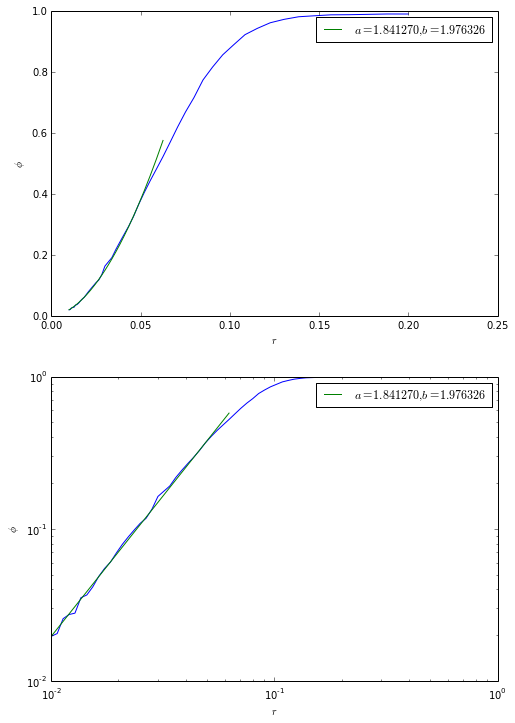
\includegraphics[width=10cm]{../img/r_phi_1_power.png}
        \caption{図\ref{fig:f16}の$0<r<0.07$の範囲をべき乗に近似したもの}
        \label{fig:f17}
    \end{center}
\end{figure}

また,これはS字型の曲線(シグモイド曲線)なので,その代表的な関数系である
\begin{eqnarray}\phi (r) = 1 - \exp \left[ -  \left( \frac{r}{\omega} \right)^{2} \right]\label{eq:e4}
\end{eqnarray}
としてパラメータ$\omega$に関して最小2乗法でフィッティングを行った。このときは先ほどの場合とは異なり,$r$の比較的大きい領域のデータを含んでいてもよい。得られたパラメータの値は$\omega=0.0715$ほどであり,図\ref{fig:f17}でべきで近似した場合に比べて,よくフィッティングできている。
\begin{figure}[H]
    \begin{center}
        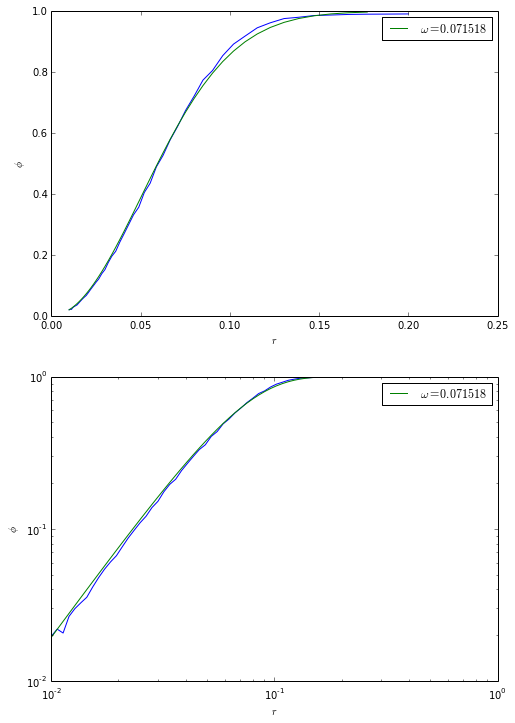
\includegraphics[width=10cm]{../img/r_phi_1_sigmoid.png}
        \caption{図\ref{fig:f16}をシグモイド曲線(\ref{eq:e4})に近似したもの}
        \label{fig:f18}
    \end{center}
\end{figure}
また,(\ref{eq:e4})式は$\phi = 1- (\text{クラスターの数})/(\text{点の総数})$の形との整合もとれているように思われる。

次に,$X_{i}$の数が変化したときにステップ間の平均移動距離$\phi$がどう変化するかについて見てみることにする。このとき,点$x$の総数$M$と$X_{i}$の数$N$,$X_{i}$あたりの点の数$S$の間には比例の関係($M=N\times S$)が成り立っており,$N$を増やすことと$S$を増やすことはこの場合等価であるから,より細かく値を刻むことのできる$S$を変化させたときのクラスター数との間の関係について調べた。横軸を$S$,縦軸を平均のステップ間距離$\phi$としたグラフを図\ref{fig:f19}に示す。このときの$N$は$N=6$であり,$r=0.07$で,100回の試行を平均したものとなっている。
\begin{figure}[H]
    \begin{center}
        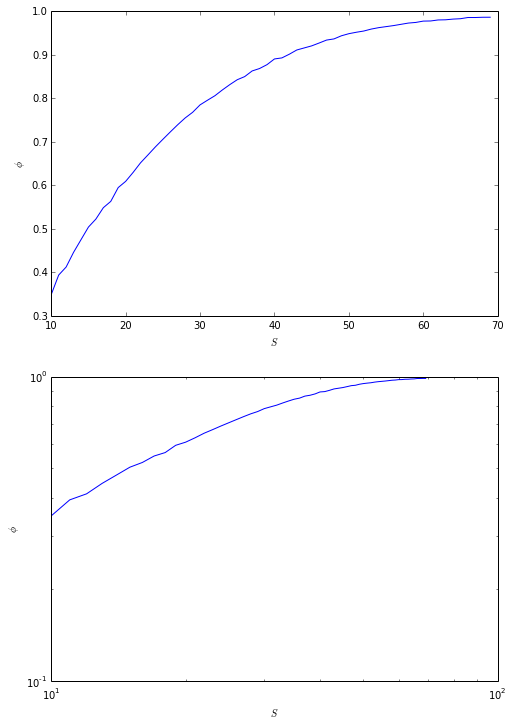
\includegraphics[width=10cm]{../img/S_phi_1.png}
        \caption{$S$を変化させたときのステップ間の平均距離}
        \label{fig:f19}
    \end{center}
\end{figure}
